% This file was created with tikzplotlib v0.10.1.
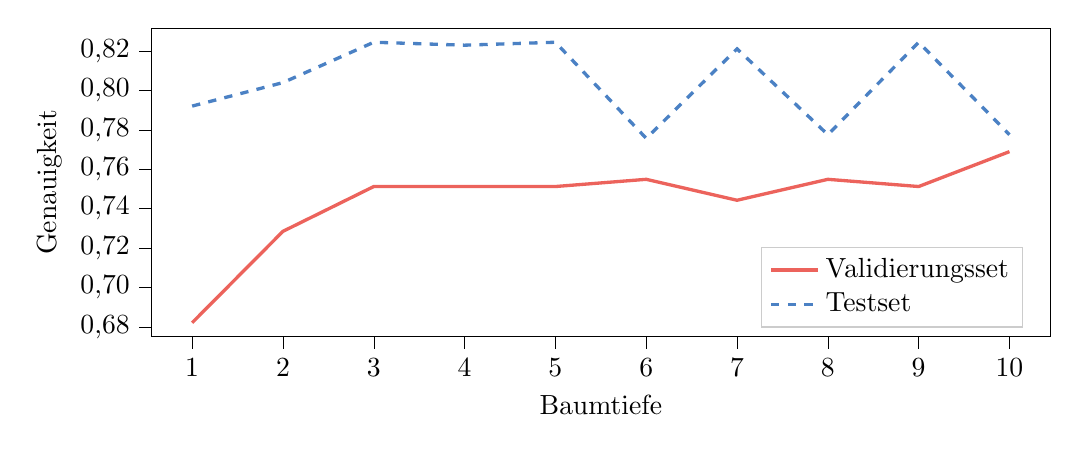
\begin{tikzpicture}

\definecolor{darkgray176}{RGB}{176,176,176}
\definecolor{lightgray204}{RGB}{204,204,204}
\definecolor{steelblue75129196}{RGB}{75,129,196}
\definecolor{tomato2369992}{RGB}{236,99,92}

\begin{axis}[
width=13cm,height=5.5cm,
legend cell align={left},
legend style={
  fill opacity=0.8,
  draw opacity=1,
  text opacity=1,
  at={(0.97,0.03)},
  anchor=south east,
  draw=lightgray204
},
tick align=outside,
tick pos=left,
x grid style={darkgray176},
xlabel={Baumtiefe},
xmin=0.55, xmax=10.45,
xtick style={color=black},
y grid style={darkgray176},
ylabel={Genauigkeit},
ymin=0.675081131767776, ymax=0.831515410958904,
ytick style={color=black},
ytick={0.66,0.68,0.7,0.72,0.74,0.76,0.78,0.8,0.82,0.84},
yticklabels={{0,66},{0,68},{0,70},{0,72},{0,74},{0,76},{0,78},{0,80},{0,82},{0,84}}
]
\addplot [very thick, tomato2369992]
table {%
1 0.682191780821918
2 0.728538812785388
3 0.751255707762557
4 0.751255707762557
5 0.751255707762557
6 0.754908675799087
7 0.744292237442922
8 0.754908675799087
9 0.751255707762557
10 0.768949771689498
};
\addlegendentry{Validierungsset}
\addplot [very thick, steelblue75129196, dashed]
table {%
1 0.79203869047619
2 0.803943452380952
3 0.824404761904762
4 0.822916666666667
5 0.824404761904762
6 0.775669642857143
7 0.821056547619048
8 0.777529761904762
9 0.824404761904762
10 0.777529761904762
};
\addlegendentry{Testset}
\end{axis}

\end{tikzpicture}
